\section{\textit{Bidirectional Encoder Representations from Transformers} \\ (BERT)}

BERT, yang merupakan singkatan dari \textit{Bidirectional Encoder Representations from Transformers}, adalah model pemrosesan bahasa alami yang diperkenalkan oleh Google pada tahun 2018 \parencite{bert}. BERT memanfaatkan arsitektur \textit{transformer}, yang telah dibahas sebelumnya, untuk memahami konteks kata dalam teks dengan cara yang lebih mendalam daripada pendekatan sebelumnya.

Salah satu keunggulan utama BERT adalah pendekatannya yang \textit{bidirectional}. Sebagai gantinya dari hanya memahami teks dari kiri ke kanan atau sebaliknya, BERT memahami konteks kata dengan mempertimbangkan informasi dari kedua arah. Ini memungkinkan model untuk memiliki pemahaman yang lebih kaya tentang makna dan nuansa dalam teks.

\begin{figure}[ht]
    \centering
    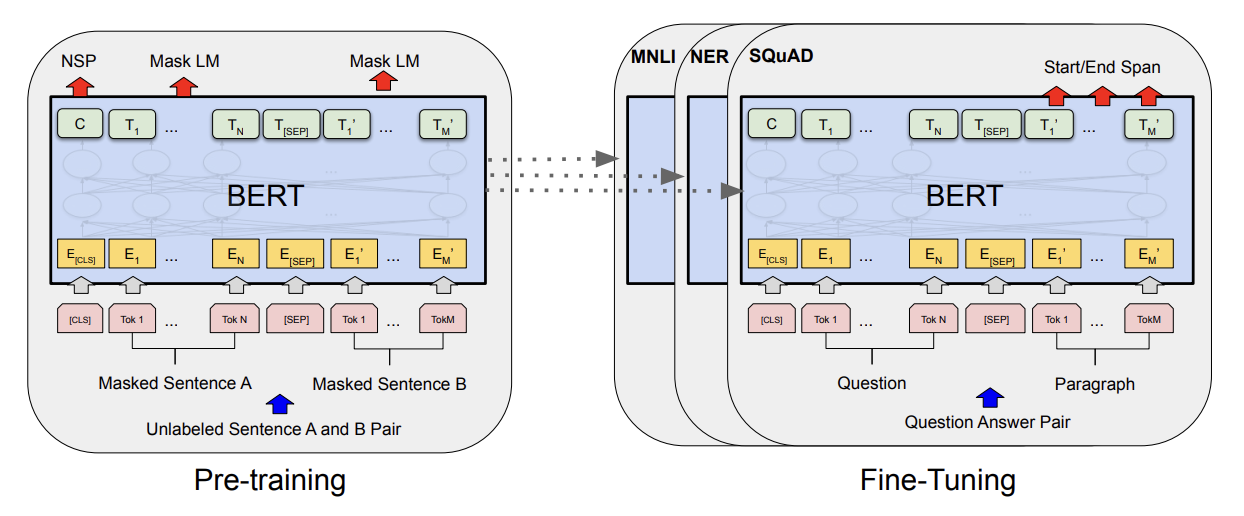
\includegraphics[width=0.8\textwidth]{chapter-2/bert.png}
    \caption{Arsitektur \textit{BERT} \parencite{bert}}
    \label{fig:bert}
\end{figure}

BERT telah dilatih pada sejumlah besar teks, yang memungkinkannya untuk mengembangkan representasi kata yang kaya dan mendalam. Ketika digunakan untuk tugas-tugas NLP spesifik, seperti klasifikasi teks atau pemahaman pertanyaan, BERT dapat disesuaikan dengan data tugas spesifik untuk mencapai kinerja yang luar biasa.
